% !TEX program = xelatex
% 需要的宏包：ctex, amsmath, amssymb, xcolor, tikz, pgfplots
\documentclass[UTF8]{ctexart}

\usepackage{amsmath,amssymb}
\usepackage[a4paper,margin=18mm]{geometry}
\usepackage{xcolor}
\usepackage{tikz}
\usepackage{pgfplots}
\pgfplotsset{compat=1.18}

\setlength{\parindent}{2em}
\setlength{\parskip}{0.4em}

\usepackage{tikz}
\usetikzlibrary{calc,intersections,angles,quotes}

\begin{document}
	\section{射影几何}
	
	文艺复兴时期，画家研究投影，研究出\textbf{射影不变性}
	
	\section{交比}
	
	\begin{figure}[htbp]
		\centering
		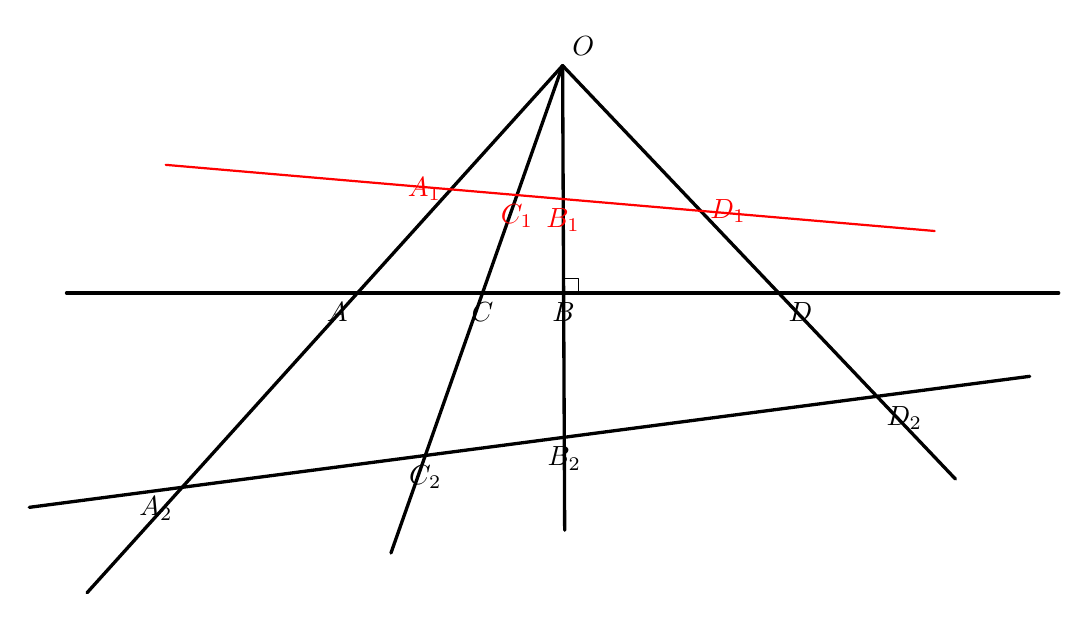
\begin{tikzpicture}[scale=1.05, line cap=round, line join=round]
			
			%====================
			% 1) 基本点与底边 A2D2（延长后的直线）
			%====================
			\coordinate (O)  at (0,4.2);
			
			% 先取底边上的两个基准点（用于确定底边方向）
			\coordinate (A2) at (-4.6,-0.9);
			\coordinate (D2) at ( 3.8, 0.2);
			
			% 在底边上再取两点，便于画出四线束
			\coordinate (B2) at ($(A2)!0.55!(D2)$);
			\coordinate (C2) at ($(A2)!0.35!(D2)$);
			
			% 将 A2D2 延长：在 A2->D2 方向上向两侧外推
			\def\tbase{0.22} % 延长比例，可调大/调小
			\coordinate (A2L) at ($(A2)!-\tbase!(D2)$);
			\coordinate (D2R) at ($(A2)!{1+\tbase}!(D2)$);
			
			% A2D2：画成延长线（无箭头）
			\draw[very thick] (A2L) -- (D2R);
			
			%====================
			% 2) 四条“射线”OA,OC,OB,OD：从 O 出发沿方向延长（不画箭头）
			%====================
			\def\k{1.25} % 射线延长倍数，可调
			\coordinate (A2e) at ($(O)!\k!(A2)$);
			\coordinate (C2e) at ($(O)!\k!(C2)$);
			\coordinate (B2e) at ($(O)!\k!(B2)$);
			\coordinate (D2e) at ($(O)!\k!(D2)$);
			
			\draw[very thick] (O) -- (A2e);
			\draw[very thick] (O) -- (C2e);
			\draw[very thick] (O) -- (B2e);
			\draw[very thick] (O) -- (D2e);
			
			%====================
			% 3) 中间水平截线：AD 也要延长（画成整条直线）
			%====================
			\path[name path=hline] (-6,1.45) -- (6,1.45);
			
			% 用延长后的射线来求交
			\path[name path=OA2] (O) -- (A2e);
			\path[name path=OC2] (O) -- (C2e);
			\path[name path=OB2] (O) -- (B2e);
			\path[name path=OD2] (O) -- (D2e);
			
			\path[name intersections={of=OA2 and hline, by=A}];
			\path[name intersections={of=OC2 and hline, by=C}];
			\path[name intersections={of=OB2 and hline, by=B}];
			\path[name intersections={of=OD2 and hline, by=D}];
			
			% AD：延长线（无箭头）
			\draw[very thick] (-6,1.45) -- (6,1.45);
			
			%====================
			% 4) 上方红色截线：产生 A1,C1,B1,D1
			%====================
			\path[name path=redline] (-4.8,3.0) -- (4.5,2.2);
			
			\path[name intersections={of=OA2 and redline, by=Aone}];
			\path[name intersections={of=OC2 and redline, by=Cone}];
			\path[name intersections={of=OB2 and redline, by=Bone}];
			\path[name intersections={of=OD2 and redline, by=Done}];
			
			\draw[thick, red] (-4.8,3.0) -- (4.5,2.2);
			
			%====================
			% 5) 点标注
			%====================
			\node[above right] at (O) {$O$};
			
			\node[below left]  at (A) {$A$};
			\node[below]       at (C) {$C$};
			\node[below]       at (B) {$B$};
			\node[below right] at (D) {$D$};
			
			\node[below left]  at (A2) {$A_2$};
			\node[below]       at (C2) {$C_2$};
			\node[below]       at (B2) {$B_2$};
			\node[below right] at (D2) {$D_2$};
			
			\node[left]  at (Aone) {\color{red}$A_1$};
			\node[below] at (Cone) {\color{red}$C_1$};
			\node[below] at (Bone) {\color{red}$B_1$};
			\node[right] at (Done) {\color{red}$D_1$};
			
			%====================
			% 6) 直角符号（示意）
			%====================
			\draw ($(B)+(0.18,0)$) -- ($(B)+(0.18,0.18)$) -- ($(B)+(0,0.18)$);
			
		\end{tikzpicture}
		
	\end{figure}
	
	\[
	\left(\frac{AC}{AB}\right)\Big/\left(\frac{BC}{BD}\right)
	\quad\text{之比，称为交比。}
	\]
	\textbf{1.\;交比具有射影不变性。}
	
	\medskip
	\noindent\textbf{（由面积比推出的交比表达式）}
	\[
	\left(\frac{AC}{AD}\right)\Big/\left(\frac{BC}{BD}\right)
	=
	\left(\frac{S_{\triangle AOC}}{S_{\triangle AOD}}\right)\Big/\left(\frac{S_{\triangle BOC}}{S_{\triangle BOD}}\right)
	\]
	
	\[
	=
	\left(\frac{\tfrac12\,OA\cdot OC\cdot\sin\angle AOC}{\tfrac12\,OA\cdot OD\cdot\sin\angle AOD}\right)
	\Bigg/
	\left(\frac{\tfrac12\,OC\cdot OB\cdot\sin\angle COB}{\tfrac12\,OD\cdot OB\cdot\sin\angle BOD}\right).
	\]
	
	
	\[
	=
	\left(\frac{\sin\angle AOC}{\sin\angle AOD}\right)\Big/\left(\frac{\sin\angle COB}{\sin\angle BOD}\right)
	=
	\frac{\sin\angle AOC}{\sin\angle AOD}\cdot\frac{\sin\angle BOD}{\sin\angle COB}.
	\]
	
	\medskip
	\noindent\textbf{二、当交比为 $-1$（调和比）}
	\[
	\overrightarrow{AC}=\lambda\,\overrightarrow{CB},\qquad
	\overrightarrow{AD}=-\lambda\,\overrightarrow{DB},
	\qquad (\lambda>0\ \text{且}\ \lambda\neq 1),
	\]
	\[
	\left|\frac{AC}{AD}\right|=\left|\frac{CB}{DB}\right|.
	\]
	
	\medskip
	\begin{center}
		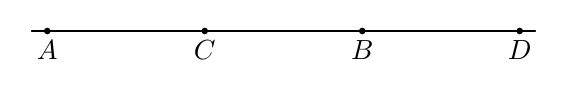
\begin{tikzpicture}[scale=1, line cap=round, line join=round]
			\draw (-0.2,0)--(6.2,0);
			\fill (0,0) circle (1.2pt) node[below] {$A$};
			\fill (2,0) circle (1.2pt) node[below] {$C$};
			\fill (4,0) circle (1.2pt) node[below] {$B$};
			\fill (6,0) circle (1.2pt) node[below] {$D$};
		\end{tikzpicture}
	\end{center}
	
	\noindent\textbf{$A,C,B,D$ 调和点列：}
	\begin{enumerate}
		\item $A,B$ 为基点，$C,D$ 为内外分点，$CD$ 调和分割 $AB$。
		\item $C,D$ 为基点，$B,A$ 为内外分点，$AB$ 调和分割 $CD$。
		\item $AB,\,CD$ 调和共轭。
	\end{enumerate}
	
	\medskip
	\noindent\textbf{③}\quad
	\[
	\frac{2}{AB}=\frac{1}{AC}+\frac{1}{AD}.
	\]
	\noindent 记：
	\[
	\frac{BC}{AC}=\frac{BD}{AD}.
	\]
	\[
	\frac{AB-AC}{AC}=\frac{AD-AB}{AD}
	\quad\Longrightarrow\quad
	\frac{AB}{AC}-1=1-\frac{AB}{AD}
	\]
	\[
	\Longrightarrow\quad
	\frac{AB}{AC}+\frac{AB}{AD}=2
	\quad\Longrightarrow\quad
	\frac{1}{AC}+\frac{1}{AD}=\frac{2}{AB}.
	\]
	
	% =========================
	
	\begin{tikzpicture}[scale=1.5, thick]
		% 定义顶点 O
		\coordinate (O) at (0,3);
		\node[above] at (O) {$O$};
		
		% 定义底部的四条射线
		\coordinate (A_inf) at (-2,0);
		\coordinate (C_inf) at (-0.8,0);
		\coordinate (B_inf) at (0.5,0);
		\coordinate (D_inf) at (2,0);
		
		% 画射线
		\draw[red] (O) -- (-2.5,-0.5);
		\draw[red] (O) -- (-1,-0.5);
		\draw[red] (O) -- (0.8,-0.5);
		\draw[red] (O) -- (2.5,-0.5);
		
		% 画第一条截线 (底部)
		\draw[red] (-2,0.5) -- (2,0.5);
		\coordinate (A) at (-1.5,0.5);
		\coordinate (C) at (-0.6,0.5);
		\coordinate (B) at (0.4,0.5);
		\coordinate (D) at (1.4,0.5);
		
		\node[below left, red] at (A) {$A$};
		\node[below, red] at (C) {$C$};
		\node[below, red] at (B) {$B$};
		\node[below right, red] at (D) {$D$};
		
		% 画第二条斜截线 (蓝色)
		\draw[blue] (-2.2,0.8) -- (1.5,2.2);
		\coordinate (Ap) at (-1.1,1.2);
		\coordinate (Cp) at (-0.35,1.5);
		\coordinate (Bp) at (0.2,1.7);
		\coordinate (Dp) at (0.55,1.85);
		
		\node[below, blue] at (Ap) {$A'$};
		\node[below, blue] at (Cp) {$C'$};
		\node[below, blue] at (Bp) {$B'$};
		\node[right, blue] at (Dp) {$D'$};
		
		% 文字标注
		\node[align=left, anchor=west] at (-1.5,4) {
			\textbf{\underline{调和点列}} $\left\{ 
			\begin{array}{l}
				1. \text{交比为 } -1 \text{ (调和平均)} \\
				2. \text{射影不变性}
			\end{array} \right.$
		};
	\end{tikzpicture}	
	
	\begin{tikzpicture}[thick, scale=1.2]
		
		% 1. 定义核心顶点 (P 和 Q)
		\coordinate (P) at (0,0);
		\coordinate (Q) at (6,8);
		
		% 2. 定义从 Q 发出的两条主干线 (蓝线)
		\path[name path=lineQ1] (Q) -- (3,-1);
		\path[name path=lineQ2] (Q) -- (9,-1);
		
		% 3. 定义 P 发出的顶部和底部射线 (用于确定 A, B, C, D)
		\path[name path=rayTop] (P) -- (10,5);   % 经过 A, E, D
		\path[name path=rayBot] (P) -- (10,0.8); % 经过 B, F, C
		
		% 4. 计算交点 A, B, C, D
		\fill [name intersections={of=lineQ1 and rayTop, by=A}] (A) circle (1.5pt) node[left] {$A$};
		\fill [name intersections={of=lineQ1 and rayBot, by=B}] (B) circle (1.5pt) node[below left] {$B$};
		\fill [name intersections={of=lineQ2 and rayTop, by=D}] (D) circle (1.5pt) node[right] {$D$};
		\fill [name intersections={of=lineQ2 and rayBot, by=C}] (C) circle (1.5pt) node[right] {$C$};
		
		% 5. 绘制对角线并确定点 O
		\draw[blue, thin] (A) -- (C);
		\draw[blue, thin] (B) -- (D);
		\path[name path=diagAC] (A) -- (C);
		\path[name path=diagBD] (B) -- (D);
		\fill [name intersections={of=diagAC and diagBD, by=O}] (O) circle (2pt) node[below right, red] {$O$};
		
		% 6. 【核心修改】定义射线 P-G-O-H，确保其经过 O
		% 使用 ($ (P)!1.5!(O) $) 来延长线段，确保覆盖到 H 点所在的区域
		\path[name path=rayMid] (P) -- ($(P)!1.8!(O)$); 
		
		% 计算 G 和 H (射线与 Q 发出的蓝线的交点)
		\fill [name intersections={of=lineQ1 and rayMid, by=G}] (G) circle (1.5pt) node[below left] {$G$};
		\fill [name intersections={of=lineQ2 and rayMid, by=H}] (H) circle (1.5pt) node[right] {$H$};
		
		% 7. 绘制穿过 Q 和 O 的中心线，并寻找 E 和 F
		\draw[name path=vertLine] ($(Q)!-0.2!(O)$) -- ($(Q)!1.5!(O)$);
		\node[right] at (Q) {$Q$};
		\fill [name intersections={of=vertLine and rayTop, by=E}] (E) circle (1.5pt) node[above left] {$E$};
		\fill [name intersections={of=vertLine and rayBot, by=F}] (F) circle (1.5pt) node[below left] {$F$};
		
		% 8. 绘制所有实线 (移除所有箭头)
		\draw[red] (P) -- (D); % 顶部红线
		\draw[black] (P) -- (H); % 中间线 (经过 G, O, H)
		\draw[red] (P) -- (C); % 底部红线
		
		\draw (A) -- (D); % 横线
		\draw (B) -- (C); % 横线
		
		\draw[blue] (Q) -- (B); % Q发出的左侧蓝线
		\draw[blue] (Q) -- (C); % Q发出的右侧蓝线
		
		% 标注顶点 P
		\node[below left] at (P) {$P$};
		
	\end{tikzpicture}
	
	
	\begin{tikzpicture}[thick, scale=1.1, font=\small]
		
		% --- 1. 定义核心坐标 ---
		% 顶点 O 位于右上方
		\coordinate (O) at (8, 6);
		% 截线的高度（y坐标）
		\def\lineY{2}
		% 定义垂足 H
		\coordinate (H) at (8, \lineY);
		
		% --- 2. 绘制水平截线 (红线) ---
		\draw[red, line width=0.8pt] (0, \lineY) -- (10, \lineY);
		\node[red, below right] at (6.5, \lineY) {调和点列};
		
		% --- 3. 计算并绘制线束 ---
		% 根据图中比例，手动设定 A, B, C, D 的横坐标
		\coordinate (A) at (1, \lineY);
		\coordinate (B) at (3.5, \lineY);
		\coordinate (C) at (5.5, \lineY);
		\coordinate (D) at (7, \lineY);
		
		% 绘制四条线束 (蓝线)
		\draw[blue] (O) -- ($(O)!1.2!(A)$);
		\draw[blue] (O) -- ($(O)!1.2!(B)$);
		\draw[blue] (O) -- ($(O)!1.2!(C)$);
		\draw[blue] (O) -- ($(O)!1.2!(D)$);
		
		% --- 4. 标注点与斜率标识 ---
		% 顶点 O
		\fill[blue] (O) circle (1.5pt) node[right, black] {$O$};
		
		% 交点 A, B, C, D
		\foreach \p in {A,B,C,D} {
			\fill[red] (\p) circle (1.5pt);
			\node[below left, black] at (\p) {$\p$};
		}
		
		% 标注 k1, k2, k3, k4
		\node[above left] at ($(O)!0.6!(A)$) {$k_1$};
		\node[above left] at ($(O)!0.6!(B)$) {$k_2$};
		\node[above left] at ($(O)!0.5!(C)$) {$k_3$};
		\node[left] at ($(O)!0.5!(D)$) {$k_4$};
		
		% --- 5. 绘制垂直高度 h ---
		\draw[dashed, red] (O) -- (H);
		\fill[black] (H) circle (1.2pt) node[below] {$H$};
		\node[right] at ($(O)!0.5!(H)$) {$h$};
		
		% --- 6. 旁边的文字标注 (可选) ---
		\node[anchor=west, align=left] at (9, 5) {
			$OA, OB, OC, OD$ \\
			\textbf{调和线束}
		};
		
		% 底部的调和比公式还原
		\node[below] at (3.5, 0.5) {$\displaystyle \frac{AB}{AD} = \frac{BC}{CD}$};
		
	\end{tikzpicture}
	
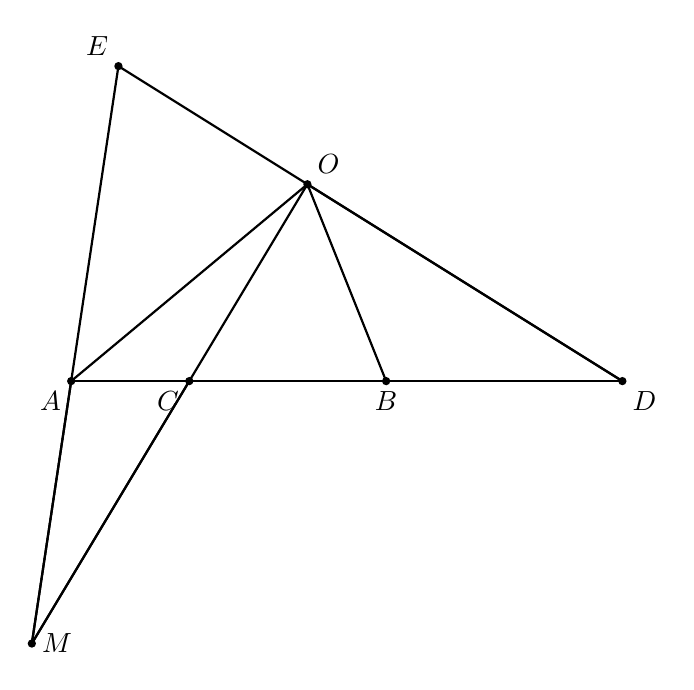
\begin{tikzpicture}[line join=round, line cap=round, thick]
	
	% --- 1. 定义核心坐标 ---  
	% 设定基线上的点 (根据图片比例调整)
	\coordinate (A) at (0,0);
	\coordinate (C) at (1.5,0);
	\coordinate (B) at (4,0);
	\coordinate (D) at (7,0);
	
	% 设定顶点 O
	\coordinate (O) at (3,2.5);
	
	% --- 2. 满足 E, O, D 三点共线 ---
	% 使用 calc 库或者简单的位似变换，让 E 落在 DO 的延长线上
	% 这里将 E 设定在从 D 穿过 O 之后的一段距离
	\coordinate (E) at ($(D)!1.6!(O)$); 
	
	% --- 3. 计算交点 M ---
	% M 是直线 EA 和直线 OC 的交点
	\coordinate (M) at (intersection of E--A and O--C);
	
	% --- 4. 绘制直线 ---
	% 绘制基线
	\draw (A) -- (D);
	
	% 绘制从 O 发出的线束
	\draw (O) -- (A);
	\draw (O) -- (B);
	\draw (O) -- (D); % 这条线实际上包含了线段 EO
	\draw (O) -- (M); % 这条线包含了 OC
	
	% 绘制从 E 发出的线
	\draw (E) -- (M); % 这条线包含了 EA
	\draw (E) -- (D); % 明确连接 E, O, D 的共线长线
	
	% 为了还原图片中 M 在下方的视觉效果，稍微延长线段
	\draw (A) -- (M);
	\draw (C) -- (M);
	
	% --- 5. 标注节点 ---
	% 这里的标记位置根据图片视觉进行了微调
	\fill (A) circle (1.5pt) node[below left] {$A$};
	\fill (B) circle (1.5pt) node[below] {$B$};
	\fill (C) circle (1.5pt) node[below left] {$C$};
	\fill (D) circle (1.5pt) node[below right] {$D$};
	\fill (O) circle (1.5pt) node[above right] {$O$};
	\fill (E) circle (1.5pt) node[above left] {$E$};
	\fill (M) circle (1.5pt) node[right] {$M$};
	
\end{tikzpicture}
	
	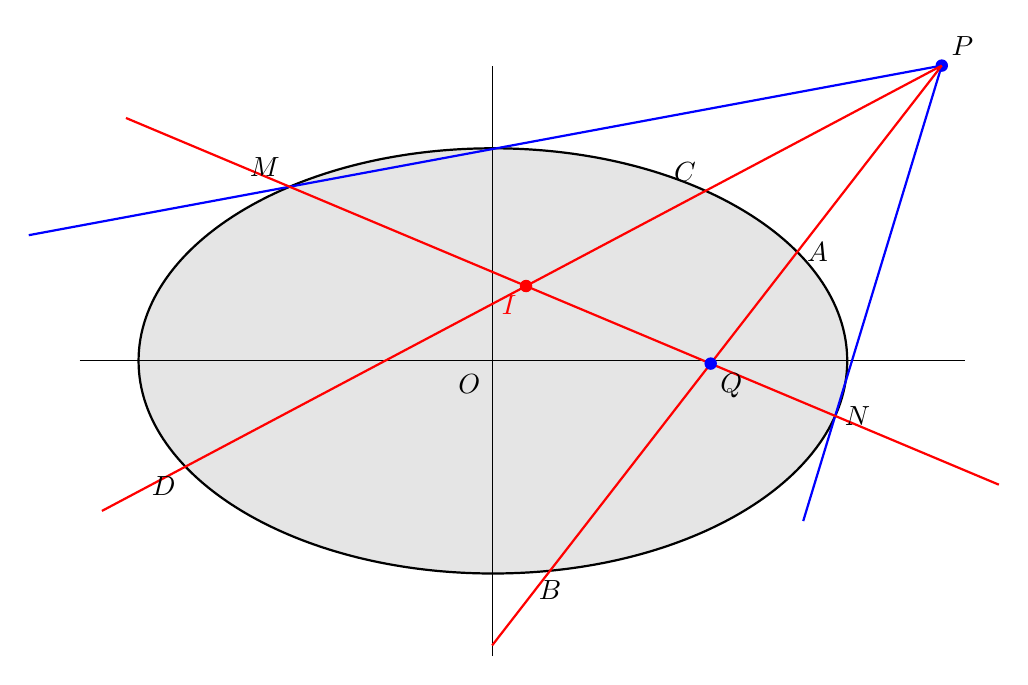
\begin{tikzpicture}[scale=1.5]
		% 0. 需在导言区引用：\usetikzlibrary{intersections, calc}
		
		% 1. 绘制灰色填充的椭圆
		\def\ea{3} \def\eb{1.8}
		\fill[gray!20] (0,0) ellipse ({\ea} and {\eb});
		\draw[thick, name path=ellipse] (0,0) ellipse ({\ea} and {\eb});
		
		% 2. 绘制坐标轴 (保留轴线，去掉箭头和标注)
		\draw (-3.5,0) -- (4,0);
		\draw (0,-2.5) -- (0,2.5);
		\node at (-0.2,-0.2) {$O$};
		
		% 3. 定义切点 M 和 N，并由切线交点确定极点 P
		\coordinate (M) at ({3*cos(125)}, {1.8*sin(125)});
		\coordinate (N) at ({3*cos(-15)}, {1.8*sin(-15)});
		
		% P点位置
		\coordinate (P) at (3.8, 2.5); 
		
		% 绘制蓝色切线 (PM 和 PN)
		\draw[blue, thick] (P) -- ($(P)!1.4!(M)$);
		\draw[blue, thick] (P) -- ($(P)!1.3!(N)$);
		\node[above right] at (P) {$P$};
		\fill[blue] (P) circle (1.5pt);
		
		% 4. 绘制红色极线 MN
		\draw[red, thick, name path=lineMN] ($(M)!-0.3!(N)$) -- ($(N)!-0.3!(M)$);
		\node[above left] at (M) {$M$};
		\node[right] at (N) {$N$};
		
		% 5. 绘制穿过 P 的两条红色割线，并向外延长
		% 割线1: P-C-D (向D点后延长)
		\path[name path=pathPD] (P) -- (-2.8, -1.0);
		\draw[red, thick, name intersections={of=ellipse and pathPD, by={C,D}}] 
		(P) -- ($(D)!-0.8cm!(P)$);
		\node[above left] at (C) {$C$};
		\node[below left] at (D) {$D$};
		
		% 割线2: P-A-B (向B点后延长)
		\path[name path=pathPB] (P) -- (0.0, -2.4);
		\draw[red, thick, name intersections={of=ellipse and pathPB, by={A,B}}] 
		(P) -- ($(B)!-0.8cm!(P)$);
		\node[right] at (A) {$A$};
		\node[below] at (B) {$B$};
		
		% 6. 计算并标注交点 I 和 Q (严格交于极线 MN)
		\path [name intersections={of=pathPD and lineMN, by={I}}];
		\fill[red] (I) circle (1.5pt) node[below left] {$I$};
		
		% Q 是直线 PB 与 极线 MN 的交点
		\path [name intersections={of=pathPB and lineMN, by={Q}}];
		\fill[blue] (Q) circle (1.5pt) node[below right, black] {$Q$};
		
	\end{tikzpicture}
	
	
	%%%%%%%%%%%%%%%
	\begin{tikzpicture}[scale=1.2, >=stealth]
		% 1. 画布裁剪
		\clip (-3.5, -3) rectangle (5.5, 3.5);
		
		\def\a{2.5}
		\def\b{1.5}
		
		% 2. 坐标轴
		\draw[->, gray!50, thin] (-3.2,0) -- (5,0) node[right] {$x$};
		\draw[->, gray!50, thin] (0,-2.5) -- (0,3) node[above] {$y$};
		
		% 3. 椭圆
		\draw[thick, red, name path=ellipse] (0,0) circle [x radius=\a, y radius=\b];
		\fill[red, opacity=0.05] (0,0) circle [x radius=\a, y radius=\b];
		
		% 4. 设定点 P
		\coordinate (P) at (3.5, 2.5); 
		\fill[red] (P) circle (1.5pt) node[above right] {$P$};
		
		% 5. 构造割线并命名路径 (延长路径确保能与极线相交)
		\path[name path=linePAB] (P) -- ($(P)!1.8!(-2, -1.2)$);
		\path [name intersections={of=ellipse and linePAB, by={A,B}}];
		\draw[blue!70, thin] (P) -- (B);
		
		\path[name path=linePCD] (P) -- ($(P)!1.8!(0.5, -2.5)$);
		\path [name intersections={of=ellipse and linePCD, by={C,D}}];
		\draw[blue!70, thin] (P) -- (D);
		
		% 6. 计算交点 M 和 N
		\coordinate (N) at (intersection of A--D and B--C);
		\coordinate (M) at (intersection of A--C and B--D);
		
		% 7. 绘制极线 MN (定义为 path 以便求交点)
		\def\ext{2.5} % 延伸系数
		\path[name path=polarLine] ($(M)!\ext!(N)$) -- ($(N)!\ext!(M)$);
		\draw[orange, thick] ($(M)!\ext!(N)$) -- ($(N)!\ext!(M)$) node[below] {极线 $l$};
		
		% 8. --- 关键修正：计算 E 和 F ---
		% E 是极线与割线 PAB 的交点
		\fill [name intersections={of=polarLine and linePAB, by={E}}] (E) circle (1.5pt) node[left, xshift=-2pt] {$E$};
		
		% F 是极线与割线 PCD 的交点
		\fill [name intersections={of=polarLine and linePCD, by={F}}] (F) circle (1.5pt) node[below right] {$F$};
		
		% 9. 绘制辅助线
		\draw[black, dashed] (A) -- (D);
		\draw[black, dashed] (B) -- (C);
		\draw[black] (A) -- (M); 
		\draw[black] (B) -- (M); 
		
		% 10. 标注剩余点
		\fill (N) circle (1.5pt) node[below left] {$N$};
		\fill (M) circle (1.5pt) node[right, xshift=2pt] {$M$};
		
		\node[above] at (A) {$A$};
		\node[left] at (B) {$B$};
		\node[right] at (C) {$C$};
		\node[below] at (D) {$D$};
		
	\end{tikzpicture}
\end{document}